\documentclass[
  stu,
  longtable,
  nolmodern,
  notxfonts,
  notimes,
  colorlinks=true,linkcolor=blue,citecolor=blue,urlcolor=blue]{apa7}

\usepackage{amsmath}
\usepackage{amssymb}



\usepackage[bidi=default]{babel}
\babelprovide[main,import]{spanish}


% get rid of language-specific shorthands (see #6817):
\let\LanguageShortHands\languageshorthands
\def\languageshorthands#1{}

\RequirePackage{longtable}
\RequirePackage{threeparttablex}

\makeatletter
\renewcommand{\paragraph}{\@startsection{paragraph}{4}{\parindent}%
	{0\baselineskip \@plus 0.2ex \@minus 0.2ex}%
	{-.5em}%
	{\normalfont\normalsize\bfseries\typesectitle}}

\renewcommand{\subparagraph}[1]{\@startsection{subparagraph}{5}{0.5em}%
	{0\baselineskip \@plus 0.2ex \@minus 0.2ex}%
	{-\z@\relax}%
	{\normalfont\normalsize\bfseries\itshape\hspace{\parindent}{#1}\textit{\addperi}}{\relax}}
\makeatother




\usepackage{longtable, booktabs, multirow, multicol, colortbl, hhline, caption, array, float, xpatch}
\setcounter{topnumber}{2}
\setcounter{bottomnumber}{2}
\setcounter{totalnumber}{4}
\renewcommand{\topfraction}{0.85}
\renewcommand{\bottomfraction}{0.85}
\renewcommand{\textfraction}{0.15}
\renewcommand{\floatpagefraction}{0.7}

\usepackage{tcolorbox}
\tcbuselibrary{listings,theorems, breakable, skins}
\usepackage{fontawesome5}

\definecolor{quarto-callout-color}{HTML}{909090}
\definecolor{quarto-callout-note-color}{HTML}{0758E5}
\definecolor{quarto-callout-important-color}{HTML}{CC1914}
\definecolor{quarto-callout-warning-color}{HTML}{EB9113}
\definecolor{quarto-callout-tip-color}{HTML}{00A047}
\definecolor{quarto-callout-caution-color}{HTML}{FC5300}
\definecolor{quarto-callout-color-frame}{HTML}{ACACAC}
\definecolor{quarto-callout-note-color-frame}{HTML}{4582EC}
\definecolor{quarto-callout-important-color-frame}{HTML}{D9534F}
\definecolor{quarto-callout-warning-color-frame}{HTML}{F0AD4E}
\definecolor{quarto-callout-tip-color-frame}{HTML}{02B875}
\definecolor{quarto-callout-caution-color-frame}{HTML}{FD7E14}

%\newlength\Oldarrayrulewidth
%\newlength\Oldtabcolsep


\usepackage{hyperref}




\providecommand{\tightlist}{%
  \setlength{\itemsep}{0pt}\setlength{\parskip}{0pt}}
\usepackage{longtable,booktabs,array}
\usepackage{calc} % for calculating minipage widths
% Correct order of tables after \paragraph or \subparagraph
\usepackage{etoolbox}
\makeatletter
\patchcmd\longtable{\par}{\if@noskipsec\mbox{}\fi\par}{}{}
\makeatother
% Allow footnotes in longtable head/foot
\IfFileExists{footnotehyper.sty}{\usepackage{footnotehyper}}{\usepackage{footnote}}
\makesavenoteenv{longtable}

\usepackage{graphicx}
\makeatletter
\def\maxwidth{\ifdim\Gin@nat@width>\linewidth\linewidth\else\Gin@nat@width\fi}
\def\maxheight{\ifdim\Gin@nat@height>\textheight\textheight\else\Gin@nat@height\fi}
\makeatother
% Scale images if necessary, so that they will not overflow the page
% margins by default, and it is still possible to overwrite the defaults
% using explicit options in \includegraphics[width, height, ...]{}
\setkeys{Gin}{width=\maxwidth,height=\maxheight,keepaspectratio}
% Set default figure placement to htbp
\makeatletter
\def\fps@figure{htbp}
\makeatother







\usepackage{newtx}

\defaultfontfeatures{Scale=MatchLowercase}
\defaultfontfeatures[\rmfamily]{Ligatures=TeX,Scale=1}





\title{Análisis Estadístico Descriptivo: Fumadores, Correlación Entre
Edad y Cigarros Fumados al Día, Diferencias de Consumo Entre Hombres y
Mujeres}


\shorttitle{Análisis Estadístico Descriptivo de 1932 Fumadores}


\usepackage{etoolbox}


\course{Computación I}
\professor{Jesús Ochoa}
\duedate{12/7/2024}







\authorsnames{Armando Delfín,Eduardo Longaart,Sonia Eveligret}






\authorsaffiliations{
{Universidad Central De Venezuela},{Departamento de Estadística y
Probabilidad}}




\leftheader{Delfín, Longaart and Eveligret}



\abstract{En este trabajo de investigación se realiza un análisis
descriptivo sobre una base de datos que contiene un número de
observaciones plasmadas en un registro con 3900 hombres y mujeres
fumadores y ex-fumadores, haciendo uso de gráficos, y de estadísticas
descriptivas para obtener información con la cual posteriormente hacer
un estudio que nos permita conocer si existe una relacion entre la edad
de las personas, su sexo y el numero de cigarros que consumen por dia.
Lo que sea desea tener como resultado de este trabajo de investigación,
es una estimación básica de lo anterior mencionado partiendo desde todos
lo registros que contengan información de las personas que son fumadores
regulares, y de forma práctica, a través del uso de graficos y medidas
descriptivas, encontrar caracteristicas asociadas a quellos que consuman
mayores cantidades de cigarros diariamente.}

\keywords{Fumadores, Características, Descriptivas}

\authornote{ 

\par{       }
\par{Correspondence concerning this article should be addressed
to Armando Delfín}
}

\makeatletter
\let\endoldlt\endlongtable
\def\endlongtable{
\hline
\endoldlt
}
\makeatother

\urlstyle{same}



\makeatletter
\@ifpackageloaded{caption}{}{\usepackage{caption}}
\AtBeginDocument{%
\ifdefined\contentsname
  \renewcommand*\contentsname{Tabla de contenidos}
\else
  \newcommand\contentsname{Tabla de contenidos}
\fi
\ifdefined\listfigurename
  \renewcommand*\listfigurename{Listado de Figuras}
\else
  \newcommand\listfigurename{Listado de Figuras}
\fi
\ifdefined\listtablename
  \renewcommand*\listtablename{Listado de Tablas}
\else
  \newcommand\listtablename{Listado de Tablas}
\fi
\ifdefined\figurename
  \renewcommand*\figurename{Figura}
\else
  \newcommand\figurename{Figura}
\fi
\ifdefined\tablename
  \renewcommand*\tablename{Tabla}
\else
  \newcommand\tablename{Tabla}
\fi
}
\@ifpackageloaded{float}{}{\usepackage{float}}
\floatstyle{ruled}
\@ifundefined{c@chapter}{\newfloat{codelisting}{h}{lop}}{\newfloat{codelisting}{h}{lop}[chapter]}
\floatname{codelisting}{Listado}
\newcommand*\listoflistings{\listof{codelisting}{Listado de Listados}}
\makeatother
\makeatletter
\makeatother
\makeatletter
\@ifpackageloaded{caption}{}{\usepackage{caption}}
\@ifpackageloaded{subcaption}{}{\usepackage{subcaption}}
\makeatother

% From https://tex.stackexchange.com/a/645996/211326
%%% apa7 doesn't want to add appendix section titles in the toc
%%% let's make it do it
\makeatletter
\xpatchcmd{\appendix}
  {\par}
  {\addcontentsline{toc}{section}{\@currentlabelname}\par}
  {}{}
\makeatother

\begin{document}

\maketitle


\setcounter{secnumdepth}{-\maxdimen} % remove section numbering

\setlength\LTleft{0pt}


\section{¿De que manera se han manejado los datos
suministrados?}\label{de-que-manera-se-han-manejado-los-datos-suministrados}

El analisis exploratorio de datos definido por Jonh W. Tukey, el cual es
el tratamiento estadístico al que se someten las muestras recogidas
durante un proceso de investigación en cualquier campo científico. Antes
de manejar la base de datos, conviene analizar los datos que se
utilizaran. Esto permite observar las caracteristicas fundamentales de
los mismos y comprender la estructura del conjuto de los datos,
identificando la variable que se tiene como objetivo y explorando las
posibles técnicas de modelado. (Tukey, J.W, 1977)

En este trabajo de investigacion se extrajo toda la informacion
necesaria de la base de datos de la siguiente manera:

Lo primero que se llevó a cabo fue observar como se comportaban los
datos y si dentro de la base de datos habian registros con valores nulos
o valores atípicos. En el caso de la columna que contiene a la variable,
cigarros consumidos al día, se encontraban 14 registros con valores
nulos, y más de 40 datos atípicos, por encima de 35 cigarros fumados
diariamente, valor que fue definido como el límite superior de la
distribución por medio de gráficos de caja y bigote.

Una vez explorada la base de datos lo siguiente a realizar fue la
depuración de esta, empleando el método de remplazar dichos valores
nulos por la media aritmética de la variable en estudio, y para los
valores atípicos por encima del límite superior, 35, contarlos como
registros de personas que fuman exactamente 35 cigarros al día.

Luego de hacer este proceso de depuración, se estudiaron a las variables
sexo, y edad, para determinar que tanto abarcaban esta dos variables
dentro de la base de datos, ordenándolas de forma ascendente para hacer
mas fácil el manejo de dichas variables dentro de la base de datos.

Al momento de finalizar todo el proceso de filtrado, depuración y
ordenamiento de los registros, el siguiente paso fue realizar gráficos
que facilitaran las interpretaciones de los datos y asi poder transmitir
de forma clara y concisa, todos los resultados obtenidos de la
investigación.

\section{Análisis Descriptivo}\label{anuxe1lisis-descriptivo}

A continuacion, en las siguientes tablas se muestran estadísticas
descriptivas para las variables en estudio, Toda la informacion respecto
a los datos a manejar fue extraída de
\url{https://www.kaggle.com/datasets/jacepranter/smoker-health-data,} de
la cual se estudia solo a los 1932 fumadores activos de entre los 3900
registros que incluyen ex-fumadores.

\begin{itemize}
\item
  En promedio, los fumadores consumen 18 cigarros diariamente, con una
  desviación estándar de 9 cigarros. Menos del 25\% de ellos fuma más de
  20 cigarros (un paquete) por día. La distribución es asimétrica
  positiva, y leptocúrtica.
\item
  En promedio, los fumadores tienen 48 años de edad, con una desviación
  estándar de 8 años. El 75\% de ellos tiene 53 años o menos. La
  distribución es asimétrica positiva , y leptocúrtica.
\item
  De todas las personas en observación, 1105 son de sexo masculino, y
  827 de sexo femenino. Representando el 57\% y 43\% respectivamente.
\end{itemize}

\begin{longtable}[]{@{}
  >{\raggedright\arraybackslash}p{(\columnwidth - 14\tabcolsep) * \real{0.1562}}
  >{\raggedright\arraybackslash}p{(\columnwidth - 14\tabcolsep) * \real{0.1562}}
  >{\raggedright\arraybackslash}p{(\columnwidth - 14\tabcolsep) * \real{0.2031}}
  >{\raggedright\arraybackslash}p{(\columnwidth - 14\tabcolsep) * \real{0.0781}}
  >{\raggedright\arraybackslash}p{(\columnwidth - 14\tabcolsep) * \real{0.0781}}
  >{\raggedright\arraybackslash}p{(\columnwidth - 14\tabcolsep) * \real{0.0781}}
  >{\raggedright\arraybackslash}p{(\columnwidth - 14\tabcolsep) * \real{0.0938}}
  >{\raggedright\arraybackslash}p{(\columnwidth - 14\tabcolsep) * \real{0.1562}}@{}}
\caption{Estadística Descriptiva Sobre las Variables
Cuantitativas}\tabularnewline
\toprule\noalign{}
\begin{minipage}[b]{\linewidth}\raggedright
Variable
\end{minipage} & \begin{minipage}[b]{\linewidth}\raggedright
Promedio
\end{minipage} & \begin{minipage}[b]{\linewidth}\raggedright
D. Estandar
\end{minipage} & \begin{minipage}[b]{\linewidth}\raggedright
Q1
\end{minipage} & \begin{minipage}[b]{\linewidth}\raggedright
Q2
\end{minipage} & \begin{minipage}[b]{\linewidth}\raggedright
Q3
\end{minipage} & \begin{minipage}[b]{\linewidth}\raggedright
C.S
\end{minipage} & \begin{minipage}[b]{\linewidth}\raggedright
Kurtosis
\end{minipage} \\
\midrule\noalign{}
\endfirsthead
\toprule\noalign{}
\begin{minipage}[b]{\linewidth}\raggedright
Variable
\end{minipage} & \begin{minipage}[b]{\linewidth}\raggedright
Promedio
\end{minipage} & \begin{minipage}[b]{\linewidth}\raggedright
D. Estandar
\end{minipage} & \begin{minipage}[b]{\linewidth}\raggedright
Q1
\end{minipage} & \begin{minipage}[b]{\linewidth}\raggedright
Q2
\end{minipage} & \begin{minipage}[b]{\linewidth}\raggedright
Q3
\end{minipage} & \begin{minipage}[b]{\linewidth}\raggedright
C.S
\end{minipage} & \begin{minipage}[b]{\linewidth}\raggedright
Kurtosis
\end{minipage} \\
\midrule\noalign{}
\endhead
\bottomrule\noalign{}
\endlastfoot
C.D & 17.9 & 9.43 & 10 & 20 & 20 & 0.07 & 2.30 \\
EDAD & 47.7 & 7.97 & 41 & 46 & 53 & 0.51 & 2.40 \\
\end{longtable}

\begin{longtable}[]{@{}
  >{\raggedright\arraybackslash}p{(\columnwidth - 6\tabcolsep) * \real{0.2394}}
  >{\raggedright\arraybackslash}p{(\columnwidth - 6\tabcolsep) * \real{0.2394}}
  >{\raggedright\arraybackslash}p{(\columnwidth - 6\tabcolsep) * \real{0.2394}}
  >{\raggedright\arraybackslash}p{(\columnwidth - 6\tabcolsep) * \real{0.2817}}@{}}
\caption{Frecuencias Relativas de los Fumadores Respecto a su
Sexo}\tabularnewline
\toprule\noalign{}
\begin{minipage}[b]{\linewidth}\raggedright
Sexo
\end{minipage} & \begin{minipage}[b]{\linewidth}\raggedright
Frecuencia Absoluta
\end{minipage} & \begin{minipage}[b]{\linewidth}\raggedright
Frecuencia Relativa
\end{minipage} & \begin{minipage}[b]{\linewidth}\raggedright
Frecuencia Relativa Porcentual
\end{minipage} \\
\midrule\noalign{}
\endfirsthead
\toprule\noalign{}
\begin{minipage}[b]{\linewidth}\raggedright
Sexo
\end{minipage} & \begin{minipage}[b]{\linewidth}\raggedright
Frecuencia Absoluta
\end{minipage} & \begin{minipage}[b]{\linewidth}\raggedright
Frecuencia Relativa
\end{minipage} & \begin{minipage}[b]{\linewidth}\raggedright
Frecuencia Relativa Porcentual
\end{minipage} \\
\midrule\noalign{}
\endhead
\bottomrule\noalign{}
\endlastfoot
M & 1105 & 0.57 & 57\% \\
F & 827 & 0.43 & 43\% \\
TOTAL & 1932 & 1 & 1 \\
\end{longtable}

\subsection{Análisis Bivariante: ¿Existe Relacion Entre la Edad de los
Fumadores y la Cantidad de Cigarros que Consumen al
día?}\label{anuxe1lisis-bivariante-existe-relacion-entre-la-edad-de-los-fumadores-y-la-cantidad-de-cigarros-que-consumen-al-duxeda}

A traves del análisis descriptivo bivariante (coeficiente de correlacion
de Pearson) y el uso de graficos se determino que existe correlacion
inversa entre el número de cigarros que fuma una persona y su edad

\begin{longtable}[]{@{}cc@{}}
\toprule\noalign{}
Covarianza & Índice de Correlación \\
\midrule\noalign{}
\endhead
\bottomrule\noalign{}
\endlastfoot
-5.30 & -0.07 \\
\end{longtable}

La covarianza entre las dos variables, edad, y cigarros consumidos al
día, tienen un valor de covarianza negativo, lo que significa que tienen
una relación negativa o inversa. A su vez, el índice de correlación, el
cual nos indica la fuerza de la relación negativa antes descubierta es
de -0.07. Teniendo en cuenta que una relación inversa puede llegar a un
máximo de -1, ésta correlación parece ser muy tenue.

Para observar estas dos variables gráficamente, nos referimos a la
siguiente figura

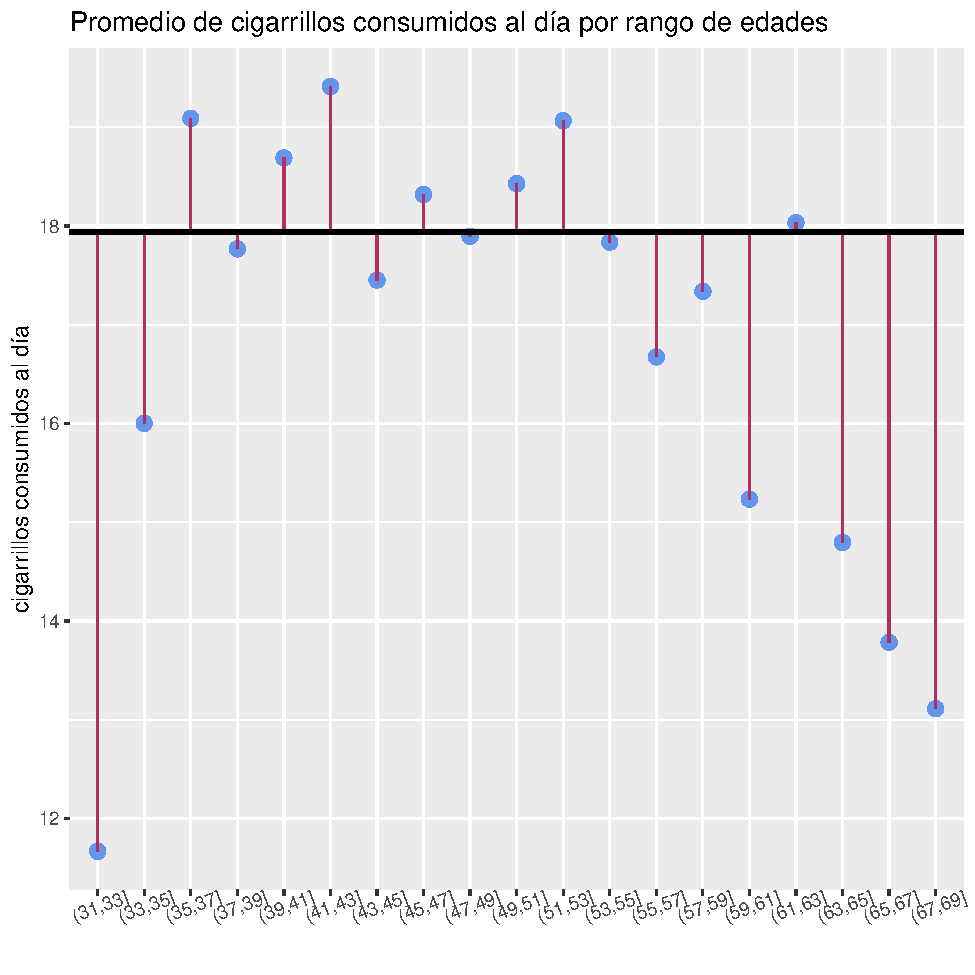
\includegraphics{Plantilla_Apa_files/figure-pdf/unnamed-chunk-1-1.pdf}

En este gráfico se muestra la correlación lineal, viendo como se
distancian las medias aritméticas de cada intervalo de edad respecto a
la media general extraída en la primera tabla, 17.9 cigarros de media.
Observamos que las medias más altas se encuentran en la parte izuierda
del gráfico, es decir que le pertenecen en los intervalos de edades que
comprenden a las personas más relativamente jóvenes en estudio. A partir
de los 55 años, se puede apreciar un declive lineal en cuanto a los
promedios de cigarros fumados al día, lo que se corresponde con las
medidas númericas descriptivas de covariaza y correlación negativa
halladas previamente.

\subsection{Cantidad de cigarros que consumen las personas dependiendo
de su
sexo}\label{cantidad-de-cigarros-que-consumen-las-personas-dependiendo-de-su-sexo}

De manera visual indicaremos que sexo dentro de la base datos consumen
una mayor cantidad de cigarros por día, a través del análisis
descriptivo y el gráfico que nos indica que generalmente el sexo más
propenso a consumir una mayor cantidad de cigarros al dia son los
hombres en observación, comparado a la distribución conformada por las
mujeres.

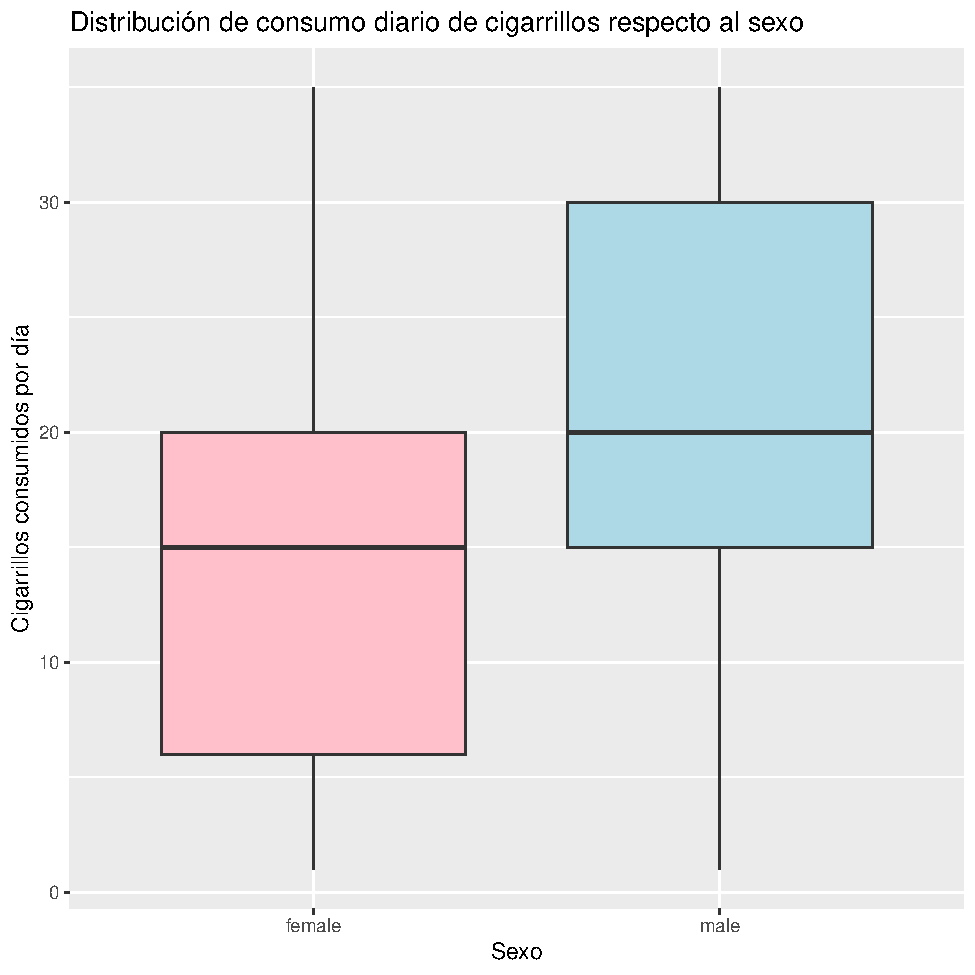
\includegraphics{Plantilla_Apa_files/figure-pdf/unnamed-chunk-2-1.pdf}

Este gráfico emplea el poderoso `five point summary' (Tukey, 1977) a
través de modelos de cajas y bigotes. Podemos observar , que el tercer
cuartil de la distribución de las mujeres fumadoras es igual a la
mediana de los hombres; 20 cigarros al día. De esto podemos derivar que
menos del 25\% de las mujeres fumadoras en observación consumen
cantidades mayores a las de un paquete estándar de 20 cigarros,
contrastado con que, por el otro lado, el 50\% de los hombres observados
fuman 20 cigarros o más. Fumar más de un paquete por día perece ser
mucho más común entre los hombres fumadores obseravdos.

\subsection{Conclusión}\label{conclusiuxf3n}

Dentro de este análisis estadistico descriptivo se han obtenido como
resultados:

\begin{itemize}
\item
  Una correlacion lineal inversa en cuanto a la edad de los fumadores y
  la cantidad cde cigarros que consumen por dia. Esto quiere decir que a
  medida que la edad de los fumadores observados se incrementaba, en
  promedio, podíamos ver un ligero decrecimiento en la cantidad de
  cigarros consumidos al día. Puede ser visto tambien desde la
  perspectiva opuesta, a medida que la edad decrecía, la media de
  cigarros consumidos al día tendía a incrementarse.
\item
  Una disparidad considerable entre el consumo de cigarros por día entre
  hombres y mujeres fumadores, con una mayor proporción de hombres, el
  50\%, fumando más de un paquete (20 cigarrillos) por día, cantidades
  que a su vez, solo son correspondidas por menos de una cuarta parte,
  25\% , de las mujeres fumadoras observadas .
\end{itemize}

Así, se ha podido dar respuesta a las preguntas planteadas en este
trabajo, pudiendo resumir en que, en promedio, de entre 1932 fumadores
observados: los hombres fuman más que las mujeres, y los de una edad
determinada suelen fumar más que las personas mayores a ellos.

\subsection{Bibliografía}\label{bibliografuxeda}

Tukey, J.W (1977) \emph{Exploratory Data Analysis.}

Reading, MA: Addison-Wesley

Kaggle.com \emph{Smoker´s Health Data}

Smoker's Health Data (kaggle.com)






\end{document}
